\documentclass{report}
\usepackage{graphicx} % Required for inserting images
\usepackage{subcaption}
\usepackage{wrapfig}
\usepackage{float}
\usepackage{amssymb}
\usepackage{hyperref}
\usepackage[utf8]{inputenc}
\usepackage{amsthm} % Required for theorem environments
\usepackage{amsmath}
\usepackage{pgfplots}
\usepackage{amsthm}
\usepackage{listings}
\usepackage[numbered,framed]{matlab-prettifier}

\usetikzlibrary{arrows.meta, decorations.markings}
\usetikzlibrary{external}
\tikzexternalize[prefix=tikz-cache/]

\pgfplotsset{compat=1.18}

\title{Dynamical systems and ergodic theory}
\author{Francesco Colombo\footnote{Based on the lectures by professor Marco Lenci}}
\date{A.A. 26/27, first semester}

% Custom style for theorems (italic body)
\newtheoremstyle{myplain}
  {\topsep}{\topsep}{\itshape}{}{\bfseries}{}{5pt}
  {\thmname{#1}\thmnumber{ #2}\thmnote{ (\textbf{#3})}}

% Custom style for definitions (upright body)
\newtheoremstyle{mydefinition}
  {\topsep}{\topsep}{\normalfont}{}{\bfseries}{}{5pt}
  {\thmname{#1}\thmnumber{ #2}\thmnote{ (\textbf{#3})}}

% Apply the theorem style
\theoremstyle{myplain}
\newtheorem{proposition}{Proposition}[chapter]
\newtheorem{lemma}{Lemma}[chapter]
\newtheorem{theorem}{Theorem}[chapter]

% Apply the definition style
\theoremstyle{mydefinition}
\newtheorem{definition}{Definition}[chapter]
\newtheorem{example}{Example}[chapter]
\newtheorem{observation}{Observation}[chapter]

\providecommand*{\propositionautorefname}{Proposition}

    % Macro: phase portrait of x' = lambda x, y' = mu y
% Usage: \phaseportrait{lambda}{mu}
\newcommand{\phaseportrait}[2]{%
\begin{tikzpicture}[scale=0.75]
    % Coordinate axes (these are trajectories too, drawn in red below)
    \draw[-{Stealth}, gray] (-2.4,0) -- (2.4,0) node[right] {$x$};
    \draw[-{Stealth}, gray] (0,-2.4) -- (0,2.4) node[above] {$y$};

    \begin{scope}
        \clip (-2.2,-2.2) rectangle (2.2,2.2);

        % Trajectories in the four quadrants: (x,y) = (x0 e^{lambda t}, y0 e^{mu t})
        % The exponent is capped (min(...,3)) to avoid TeX dimension overflow;
        % the capped part lies outside the clipping box anyway.
        \foreach \sx in {1,-1} {
            \foreach \sy in {1,-1} {
                \foreach \xo/\yo in {1.2/0.4, 1.2/1.2, 0.5/1.2} {
                    % full curve
                    \draw[thin, blue!70!black, domain=-6:6, samples=200, variable=\t]
                        plot ({\sx*\xo*exp(min(#1*\t,3))}, {\sy*\yo*exp(min(#2*\t,3))});
                    % short piece starting at (x0,y0): carries the arrow (direction of increasing t)
                    \draw[thin, blue!70!black, -{Stealth[length=1.8mm]},
                          domain=0:0.2, samples=3, variable=\t]
                        plot ({\sx*\xo*exp(#1*\t)}, {\sy*\yo*exp(#2*\t)});
                }
            }
        }

        % Trajectories lying on the axes (x0,0) and (0,y0)
        \foreach \s in {1,-1} {
            \draw[thick, red!70!black, -{Stealth[length=2.2mm]},
                  domain=0:0.25, samples=3, variable=\t]
                plot ({\s*1.2*exp(#1*\t)}, 0);
            \draw[thick, red!70!black, -{Stealth[length=2.2mm]},
                  domain=0:0.25, samples=3, variable=\t]
                plot (0, {\s*1.2*exp(#2*\t)});
        }
    \end{scope}

    \fill (0,0) circle (1.5pt);
    \node[below] at (0,-2.4) {\small $\lambda=#1,\ \mu=#2$};
\end{tikzpicture}%
}

% Macro: phase portrait of z' = Bz with e^{tB} = e^{at} R_{bt}  (a != 0)
% Usage: \spiralportrait{a}{b}
% Trajectory: (x,y) = e^{at} (cos(bt), sin(bt)) * r0, i.e. r = r0 e^{at}, theta = bt.
% If a>0 the spiral starts near the origin and winds outwards;
% if a<0 it starts at the border of the picture and winds inwards.
% In both cases t runs over [0,T] so that r goes between 0.08 and 2.2.
\newcommand{\spiralportrait}[2]{%
\begin{tikzpicture}[scale=0.75]
    % Coordinate axes
    \draw[-{Stealth}, gray] (-2.4,0) -- (2.4,0) node[right] {$x$};
    \draw[-{Stealth}, gray] (0,-2.4) -- (0,2.4) node[above] {$y$};

    % Time needed to cross the annulus 0.08 < r < 2.2, and starting radius
    \pgfmathsetmacro{\T}{ln(27.5)/abs(#1)}
    \pgfmathsetmacro{\rz}{ifthenelse(#1>0,0.08,2.2)}

    % Two trajectories: the second one is the first rotated by 180 degrees
    \foreach \rot in {0,180} {
        \begin{scope}[rotate=\rot]
            \draw[thick, blue!70!black,
                  domain=0:\T, samples=300, variable=\t,
                  postaction={decorate},
                  decoration={markings,
                      mark=at position 0.35 with {\arrow{Stealth[length=2.2mm]}},
                      mark=at position 0.65 with {\arrow{Stealth[length=2.2mm]}},
                      mark=at position 0.95 with {\arrow{Stealth[length=2.2mm]}}}]
                plot ({\rz*exp(#1*\t)*cos(deg(#2*\t))},
                      {\rz*exp(#1*\t)*sin(deg(#2*\t))});
        \end{scope}
    }

    \fill (0,0) circle (1.5pt);
    \node[below] at (0,-2.4) {\small $a=#1,\ b=#2$};
\end{tikzpicture}%
}

% Macro: case a = 0, trajectories are circles run with angular velocity b
% Usage: \circleportrait{b}   (b>0 counterclockwise, b<0 clockwise)
\newcommand{\circleportrait}[1]{%
\begin{tikzpicture}[scale=0.75]
    % Coordinate axes
    \draw[-{Stealth}, gray] (-2.4,0) -- (2.4,0) node[right] {$x$};
    \draw[-{Stealth}, gray] (0,-2.4) -- (0,2.4) node[above] {$y$};

    \pgfmathsetmacro{\endangle}{ifthenelse(#1>0,360,-360)}
    \foreach \r in {0.7,1.4,2.1} {
        \draw[thick, blue!70!black,
              postaction={decorate},
              decoration={markings,
                  mark=at position 0.125 with {\arrow{Stealth[length=2.2mm]}},
                  mark=at position 0.625 with {\arrow{Stealth[length=2.2mm]}}}]
            (\r,0) arc (0:\endangle:\r);
    }

    \fill (0,0) circle (1.5pt);
    \node[below] at (0,-2.4) {\small $a=0,\ b=#1$};
\end{tikzpicture}%
}

% Macro: phase portrait of x' = lambda x + y, y' = lambda y   (Jordan block)
% Usage: \jordanportrait{lambda}
% Trajectory through (x0,y0): (x,y) = ((x0 + y0 t) e^{lambda t}, y0 e^{lambda t})
\newcommand{\jordanportrait}[1]{%
\begin{tikzpicture}[scale=0.75]
    % Coordinate axes
    \draw[-{Stealth}, gray] (-2.4,0) -- (2.4,0) node[right] {$x$};
    \draw[-{Stealth}, gray] (0,-2.4) -- (0,2.4) node[above] {$y$};

    \begin{scope}
        \clip (-2.2,-2.2) rectangle (2.2,2.2);

        % Generic trajectories, starting at (x0,y0) with y0 != 0.
        % The map (x,y) -> (-x,-y) preserves the system, so \s = -1 gives the mirrored ones.
        % The exponent is capped (min(...,3)) to avoid TeX dimension overflow;
        % the capped part lies outside the clipping box anyway.
        \foreach \s in {1,-1} {
            \foreach \xo/\yo in {-1.5/0.6, 0/0.6, 1.5/0.6, -0.8/1.5, 0.8/1.5} {
                % full curve
                \draw[thin, blue!70!black, domain=-6:6, samples=300, variable=\t]
                    plot ({\s*(\xo+\yo*\t)*exp(min(#1*\t,3))},
                          {\s*\yo*exp(min(#1*\t,3))});
                % short piece starting at (x0,y0): carries the arrow (increasing t)
                \draw[thin, blue!70!black, -{Stealth[length=1.8mm]},
                      domain=0:0.2, samples=3, variable=\t]
                    plot ({\s*(\xo+\yo*\t)*exp(#1*\t)},
                          {\s*\yo*exp(#1*\t)});
            }
        }

        % Trajectories on the x-axis (y0 = 0): the only straight-line trajectories
        \foreach \s in {1,-1} {
            \draw[thick, red!70!black] (0,0) -- (\s*2.2,0);
            \draw[thick, red!70!black, -{Stealth[length=2.2mm]},
                  domain=0:0.25, samples=3, variable=\t]
                plot ({\s*1.2*exp(#1*\t)}, 0);
        }
    \end{scope}

    \fill (0,0) circle (1.5pt);
    \node[below] at (0,-2.4) {\small $\lambda=#1$};
\end{tikzpicture}%
}

\begin{document}
\maketitle
\tableofcontents


\chapter*{Main definitions}
\section*{Fundamental definition}
\begin{definition}
    A dynamical system (DS) over the set M(usually called phase space or reference space) is a family ${\phi^t}_{t\in\mathbb{G}}$ of transformations $\phi^t:M\rightarrow M$ with the (semi)group property:
    \begin{equation*}
        \phi^0=id_M
    \end{equation*}
    \begin{equation*}
        \phi^{t+s}=\phi^s\circ \phi^t
    \end{equation*}
    Note: $\mathbb{G}$ must be a commutative semigroup with neutral element with respect to the "+" operation. In practice, for the contents of this course, $\mathbb{G}=\mathbb{R},\,\mathbb{R}^+_0,\,\mathbb{Z},\,\mathbb{N}$
\end{definition}

\begin{observation}
Differential equations not depending on time derivatives satisfy the definition.
\end{observation}

Usually the formalism is that, say x is the state now (meaning at $t=0$), then the state at time t is given by $\phi^t(x)$. 

\begin{definition}
    If $\mathbb{G}=\mathbb{R},\mathbb{R}^+_0$, then $\phi^t$ is called the flow of the DS. if, instead, $\mathbb{G}=\mathbb{Z},\mathbb{N}$ usually you rename it as $T=\phi^1,\,n=t$ where T is called a map.
\end{definition}
\begin{observation}
    This is due to the fact that by just knowing T you can have enough information to know the future of the system, since \begin{equation*}
    \phi^t=(\phi^1)^n=\underbrace{\phi^1\circ\phi^1....\circ\phi^1}_{\text{n times}}=T^n
    \end{equation*}
\end{observation}
Note that from now on if $n$ is an integer exponent it means to use the transformation $n$ times. Also, if T is invertible(bijective) we denote, for $n\in\mathbb{Z}^+$:\begin{equation*}
    T^{-n}=\underbrace{T^{-1}\circ T^{-1}.....\circ T^{-1}}_{\text{n times}}
\end{equation*}
Observe that $\forall n,\,m\in\mathbb{Z}$:
\begin{equation*}
    T^{n+m}=T^n\circ T^m
\end{equation*}
Notice that by having T be invertible, it means that by knowing it you can also go back in time, and as such you know everything about the system; we will see both bijective and not in this course. (here he drew a figure). 
\chapter{Examples of simple dynamical systems}
\section{Important example: autonomous ODEs}
\begin{figure}[ht]
    \centering
    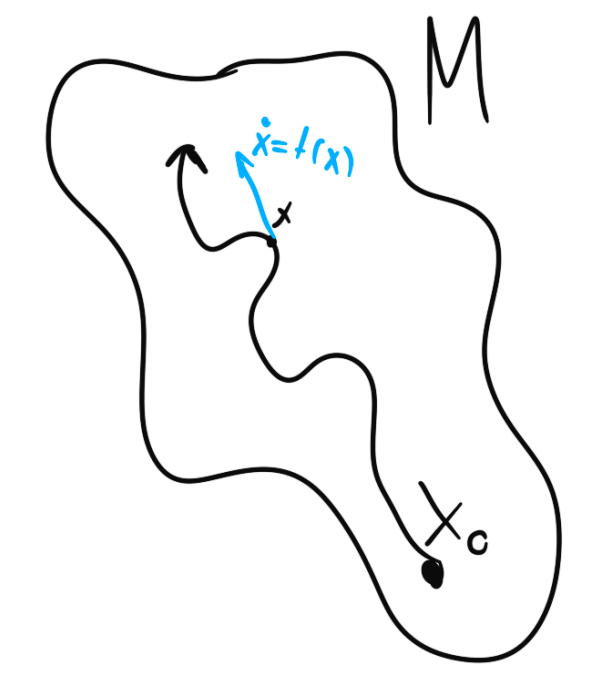
\includegraphics[width=0.3\textwidth]{img/cap1/cauchy.png}
    \caption{Representation of the quantities in an autonomous ODE.}
    \label{fig:aut_ode}
\end{figure}
The most obvious example of a dynamical system is given by an ODE, which takes the form of:
\begin{equation*}
    \dot{x}=f(x)
\end{equation*}
where $M\subseteq\mathbb{R}^d,\,f:M\rightarrow\mathbb{R}^d$. 

We are looking at a curve of which we know the first time derivative, and we know said derivative to be a function of position, but not of time, as shown in \autoref{fig:aut_ode}. 

The aforementioned problem has, potentially, infinite solutions. What interests us are what are called Cauchy problems or, more commonly,\footnote{This is true for the whole world, apart from Italy and France, which only call those Cauchy problems. The latter has obvious reasons to do so. Italy, on the other hand, hasn't got so many.} IVP, Initial Value Problems.

\begin{definition}[Cauchy problem]
    A Cauchy problem is given by the following linear system:
    \begin{equation}
    \begin{cases}
    \dot{x}=f(x) \\
    x(0)=x_0
    \end{cases}
    \label{eq:cauchy}
    \end{equation}
\end{definition}
Cauchy's theorem tells us that under some conditions, which we assume, the solution exists, and it's unique. (those conditions being that f(x) is a Lipschitz function). 

We shall start with the classic ODE example: the harmonic oscillator.

\begin{figure}[ht]
    \centering
    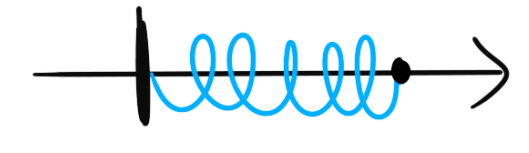
\includegraphics[width=0.3\textwidth]{img/cap1/harmonic_oscillator.png}
    \caption{Representation of a harmonic oscillator.}
    \label{fig:harmonic_oscillator}
\end{figure}

\begin{example}[Harmonic oscillator]
    The one dimensional harmonic oscillator is a physical system in which a mass is attracted to the origin by a force that depends on the distance to the origin itself, as shown in \autoref{fig:harmonic_oscillator}. This is described by:
    \begin{equation}
        \ddot{x}=-w^2x
    \end{equation}
    At first glance, it may look like it does not fit the definition of a Cauchy problem, since it is a second derivative instead of a first one. Turns out, all high order ODEs may be reduced to a single order one. 

    The trick is to rename the first derivative. in this case:
    \begin{equation*}
        \begin{cases}
            \dot{x}=v \\
            \dot{v}=-w^2x
        \end{cases}
    \end{equation*}
    Or, in matrix form:
    \begin{equation*}
        \dot{\begin{bmatrix}x \\ v\end{bmatrix}}=\begin{bmatrix} v \\ -w^2x\end{bmatrix}=f\left(\begin{bmatrix} x \\ v\end{bmatrix}\right)
    \end{equation*}
    We did increase the dimension of the phase space, but that does not get in the way of calling this a Cauchy problem.
\end{example}

Other than uniqueness and existence, we will also be implicitly assuming  all solutions to be global, i.e. defined $\forall t\in\mathbb{R}$, which is a much more restrictive condition. While finding a problem for which uniqueness and existence are not true is quite hard, the same is not true for a Cauchy problem without a global solution. Case in point:

\begin{example}[of a non global solution]
    \begin{equation*}
        \begin{cases}
            \dot{x}=x^2 \\
            x(0)=1
        \end{cases}
    \end{equation*}
    where $M=\mathbb{R}$.
    Solving it by abusing math a bit:
    \begin{equation*}
        \frac{dx}{dt}=x^2 \Leftrightarrow \frac{dx}{x^2}=dt\Leftrightarrow\int_1^x\frac{d\xi}{\xi^2}=\int_0^td\tau\Leftrightarrow\left[-\frac{1}{\xi}\right]^x_1=t  \Leftrightarrow 1-\frac{1}{x}=t\Leftrightarrow x=\frac{1}{1-t}
    \end{equation*}
    \begin{tikzpicture}
    \begin{axis}
    % Plot left branch (x < 1)
    \addplot [domain=-3:0.9, samples=100, blue, thick] {1/(1-x)};

    % Plot right branch (x > 1)
    \addplot [domain=1.1:5, samples=100, blue, thick] {1/(1-x)};

    % Draw vertical asymptote at x = 1
    \draw [dashed, red, thick] (axis cs:1,-10) -- (axis cs:1,10);
    \end{axis}
    \end{tikzpicture}

    As you can see, it blows up asymptotically at 1, so it is not a global solution.
\end{example}

We shall now see the concept of flow.

\begin{figure}[ht]
    \centering
    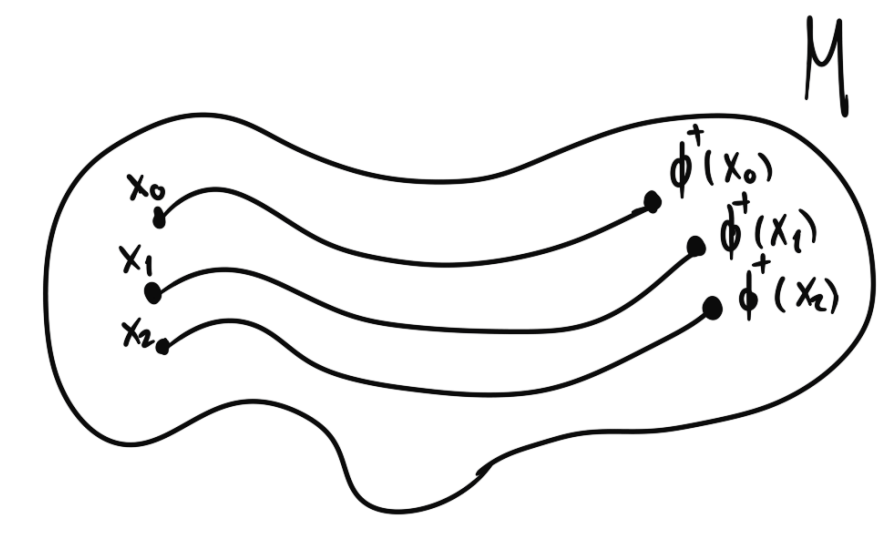
\includegraphics[width=0.5\textwidth]{img/cap1/flux.png}
    \caption{Representation of flow.}
    \label{fig:flow}
\end{figure}

\begin{definition}
    If $x(t;x_0)$ is the solution of \autoref{eq:cauchy}, the flow of such system is:
    \begin{equation}
        \phi^t(x_0)=x(t;x_0)
        \label{eq:flow}
    \end{equation}
\end{definition}

\begin{proposition}
    $\phi^t_{t\in\mathbb{R}}$, as defined in \autoref{eq:flow} satisfies the group property.
\end{proposition}

\begin{proof}
    The group properties are two:
    \begin{equation}
        \phi^0=id_M
        \label{eq:identity}
    \end{equation}
    \begin{equation}
        \phi^{t+s}=\phi^s\circ \phi^t
        \label{eq:composition}
    \end{equation}

    \autoref{eq:identity} is trivial, because by definition $\phi^0(x_0)=x_0\forall\, x_0\in M$.

    The second property is a bit harder. First of all, by definition:
    \begin{equation}
        \phi^{t+s}=\phi^t\circ\phi^s\Leftrightarrow \phi^t(\phi^s(x_0))=\phi^{t+s}(x_0)\forall x_0
        \label{eq:proof}
    \end{equation}
    We define $y_1(t)=\phi^t(\phi^s(x_0))$ and $y_2(t)=\phi^{t+s}(x_0)$. We'll prove that $y_1(t)$ and $y_2(t)$ are both solutions of the following IVP:
    \begin{equation}
        \begin{cases}
            \dot{y}(t)=f(y(t)) \\ y(0)=\phi^s(x_0) \forall s\in\mathbb{R},\ x_0\in M
        \end{cases}
    \end{equation}
    Because of Cauchy's theorem of uniqueness, if both solve the IVP, they must be equal, thus the proposition will be proved because of \autoref{eq:proof}. 

    The initial condition is true by definition:
    \begin{equation*}
        \begin{matrix}
        y_1(0)=\phi^{0}(\phi^s(x_0))=\phi^s(x_0) \cr \cr y_2(0)=\phi^{0+s}(x_0)=\phi^{s}(x_0) \cr
        \end{matrix} \Leftrightarrow y_1(0)=y_2(0)=\phi^s(x_0)\forall s\in \mathbb{R}
    \end{equation*}

    As for the other condition, for $y_1$ it's true by definition, first by the definition of $y_1$ itself, then by the definition of $\phi^t(x_0)$:
        \begin{equation*}
        \begin{aligned}
        \frac{dy_1}{dt}(t)=\frac{d\phi^t}{dt}(\phi^s(x_0))=\frac{dx(t;\,\phi_s(x_0))}{dt}= \\
        f(x(t;\,\phi^s(x_0)))=f(\phi^t(\phi^s(x_0)))=f(y_1(t))
        \end{aligned}
        \end{equation*}

    
    where x is the solution of the IVP over which the flow is defined, while f() for which $\dot{x}=f(x)$ is true.

    In the same way, by employing the definitions of $y_2$ and flow, aided by the chain rule, we may find that the temporal derivative of $y_2$ is equal to $f(y_2)$, where f() is the same as the one for which that is true for $y_1$:
        \begin{equation*}
        \begin{aligned}
        \frac{dy_2}{dt}(t)=\frac{d\phi^{t+s}}{dt}(x_0)=\frac{dx(t+s;\,x_0)}{dt}\frac{d(t+s)}{dt}= \\
        f(x(t+s;\,x_0))=f(\phi^{t+s}(x_0))=f(y_2(t))
        \end{aligned}
        \end{equation*}
    
    So, $y_1$ and $y_2$ both solve the aforementioned IVP for every t, thus we proved the proposition.


\end{proof}
Let's now look a bit into the concept of flow. The flow behaves in such a way(this is why it's called a flow!) in which it never intercepts. It looks, if drawn in a stylized way, as a series of lines that never intercept, because of the uniqueness of the solution of the Cauchy problem, as shown in \autoref{fig:flow}.

\begin{figure}[ht]
    \centering
    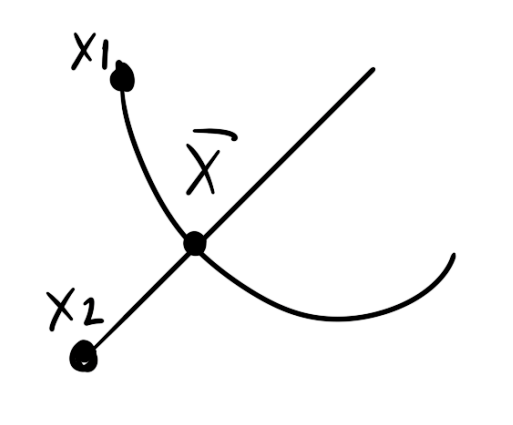
\includegraphics[width=0.3\textwidth]{img/cap1/intersection.png}
    \caption{Representation of the hypothesis used to prove \autoref{prop:intersection}.}
    \label{fig:intersection}
\end{figure}

\begin{proposition}
    We define two flows $\phi^{t_1}(x_1)$ and $\phi^{t_2}(x_2)$. If $t_1\geq t_2$ and $x_1\neq x_2$, they shall never intercept. 
    \label{prop:intersection}
\end{proposition}
\begin{proof}
    RAA\footnote{Reductio ad absurdum. I will use this to signal that I am proving by contradiction.} Assume that we have two trajectories that are completely distinct apart from one singular interception. Let's call the singular interception $\bar{x}$. The following is true by definition:
    \begin{equation*}
        \bar{x}=\phi^{t_1}(x_1)=\phi^{t_2}(x_2)
    \end{equation*}
    But then, by definition of flow:
    \begin{equation*}
        \phi^{-t_2}(\bar{x})=\phi^{-t_2}(\phi^{t_2}(\bar{x}))=x_2
    \end{equation*}
    but at the same time:
    \begin{equation*}
        \phi^{-t_2}(\bar{x})=\phi^{-t_2}(\phi^{t_1}(x_1))=\phi^{t_1-t_2}(x_1)
    \end{equation*}
    The hypothesis here that the interception is just one. Starting from said hypothesis, we found another interception, namely $x_2$. This would mean, because of the uniqueness of the solution of the Cauchy problem, that the trajectories are exactly the same: but that is impossible, because we assumed that they were distinct apart from one singular point.
\end{proof}

\begin{example}[of global solution ascertained by visual inspection]
    Suppose M is a two dimensional domain and suppose you know that at the boundary the vector field f always points inside. And suppose you know that this vector field is smooth. Then you are assured that the solution is global, because you cannot escape. 
\end{example}

Usually you can find a global solution becuase you can iteratively move inside small intervals.   

\chapter{Topological dynamics}
\chapter{Ergodic theory}
\chapter{Possible developments}
\chapter*{Appendix}
\section*{Matlab code for the logistic map}
\label{sec:matlab_cobweb}
I took the liberty to use a slightly different code from the professor for that simulation:
\begin{lstlisting}[style=Matlab-editor, caption={Logistic Map Script}]
clear all

close all

set(groot, 'defaultFigureColor', 'w', ...
    'defaultAxesColor', 'w', ...
    'defaultAxesXColor', 'k', ...
    'defaultAxesYColor', 'k', ...
    'defaultTextColor', 'k');

N=200; % number of iterations

r=2.6;

x0=0.95;


xm=linspace(0,1,100);

ym=map(r,xm);

x = zeros(1,N);

xp=zeros(1,2*N+1);

yp=zeros(1,2*N+1);

x(1)=x0; % initial condition (can be anything from 0 to 1)

xp(1)=x0;


for n = 1:N

    x(n+1)=map(r,x(n));

    xp(2*n)=xp(2*n-1);

    yp(2*n)=x(n+1);

    xp(2*n+1)=x(n+1);

    yp(2*n+1)=x(n+1);

end

% Define the double-time map function
map2 = @(r, s) map(r, map(r, s));
ym2 = map2(r, xm);

% Compute trajectory and cobweb points for the double-time map
x2 = zeros(1, N);
xp2 = zeros(1, 2*N+1);
yp2 = zeros(1, 2*N+1);
x2(1) = x0;
xp2(1) = x0;

for n = 1:N
    x2(n+1) = map2(r, x2(n));
    xp2(2*n) = xp2(2*n-1);
    yp2(2*n) = x2(n+1);
    xp2(2*n+1) = x2(n+1);
    yp2(2*n+1) = x2(n+1);
end

% Create a single figure window with subplots
figure;

% First panel: Map function and Cobweb diagram
subplot(1, 2, 1);
plot(xm, xm, 'k--', 'LineWidth', 1);     % Identity line y = x
hold on;
plot(xm, ym, 'r', 'LineWidth', 1.5);        % Single-time map curve
plot(xp, yp, 'b');                           % Single map cobweb trajectory
title('T(x)');
xlabel('x_n');
ylabel('x_{n+1}');
legend('y = x', 'Single Map', 'Cobweb 1x');
grid on;

%Second panel: Double map
%subplot(1, 3, 2);
%plot(xm, xm, 'k--', 'LineWidth', 1);     % Identity line y = x
%hold on;
%plot(xm, ym2, 'm', 'LineWidth', 1.5);       % Double-time map curve
%plot(xp2, yp2, 'g');                       % Double map cobweb trajectory
%title('T^2(x)');
%xlabel('x_n');
%ylabel('x_{n+1}');
%legend('y = x', 'Double Map', 'Cobweb 2x');
%grid on;

% Second/third panel: Time series trajectory x(n)
subplot(1, 2, 2);
plot(x, '.-');
xlim([0 200]);
title('Trajectory x(n)');
xlabel('n');
ylabel('x_n');
grid on;

function m=map(r,s)
m=r*s.*(1-s);
%    m0=r*s.*(1-s);   % this is the double-time map
%    m=r*m0.*(1-m0);
end

\end{lstlisting}

One quick note: to display also the squared map, one must uncomment the middle panel and then change all the subplot() have 3 as the middle number, and also as the last one for the trajectory panel.

\end{document}